\section{Experiments and Results}
\label{Results}

\subsection{Evaluation protocol}
We evaluate on a held-out split of ResPlan. The train/eval partition is a
deterministic seeded split over the raw plan indices, so the evaluation set is
fixed across runs and never seen during training. We hold out $10\%$ of the plans
for evaluation. Augmentation (rotations and flips) is applied only to the training
split.

We report two metrics. The first is the Fr\'echet Inception Distance
(FID)~\cite{FID}, computed on $256\times256$ rasterised renders of the plans using
InceptionV3 features. Because FID is biased on finite samples and our renders carry
some rasterisation noise, we also report an \emph{FID floor}: the FID between two
disjoint, identically distributed halves of the ground-truth set. This captures the
finite-sample and rendering noise alone and sets a conservative reference against
which the model's FID should be read. The second metric is a graph-based \emph{Compatibility} score,
following HouseDiffusion~\cite{HouseDiffusion}. We re-estimate the room-adjacency
graph from each generated plan using the same edge rules as the ResPlan graph
construction (direct, adjacency, and via-door/window connections) and count the
edge mismatches against the conditioning graph; lower is better. We run five
independent sampling passes of $1000$ plans each and report the mean and standard
deviation.

\begin{table}[t]
  \centering
  \small
  \setlength{\tabcolsep}{6pt}
  \renewcommand{\arraystretch}{1.15}
  \begin{tabular}{@{}l c c@{}}
    \toprule
    & HouseDiffusion-ResPlan & FID floor \\
    \midrule
    FID ($\downarrow$)           & $44.79 \pm 0.94$ & $16.36$ \\
    Compatibility ($\downarrow$) & $2.84 \pm 0.04$  & --- \\
    \bottomrule
  \end{tabular}
  \caption{Quantitative results on the held-out ResPlan split, as mean $\pm$ std
  over five sampling runs of $1000$ plans. The FID floor is the FID between two
  disjoint halves of the ground-truth set ($500$ renders each) and lower-bounds
  the score attainable under our finite-sample, rasterised evaluation;
  Compatibility counts graph-edge mismatches per plan.}
  \label{tab:results}
\end{table}

\subsection{Qualitative results}
We render generated plans with an architectural renderer that draws walls, door
swings, and window glyphs, so the structure of the generated layouts can be
inspected directly against ground-truth plans. Figure~\ref{fig:qualitative} shows
two held-out conditioning graphs with their ground truth (left) and a sample from
the final model (right). The generated plans recover the correct rooms and most of
the intended adjacencies, with walls, doors, and windows in plausible positions;
the main failure mode is geometric, as room outlines are looser and occasionally
overlap rather than tiling the floor cleanly.

\begin{figure}[t]
  \centering
  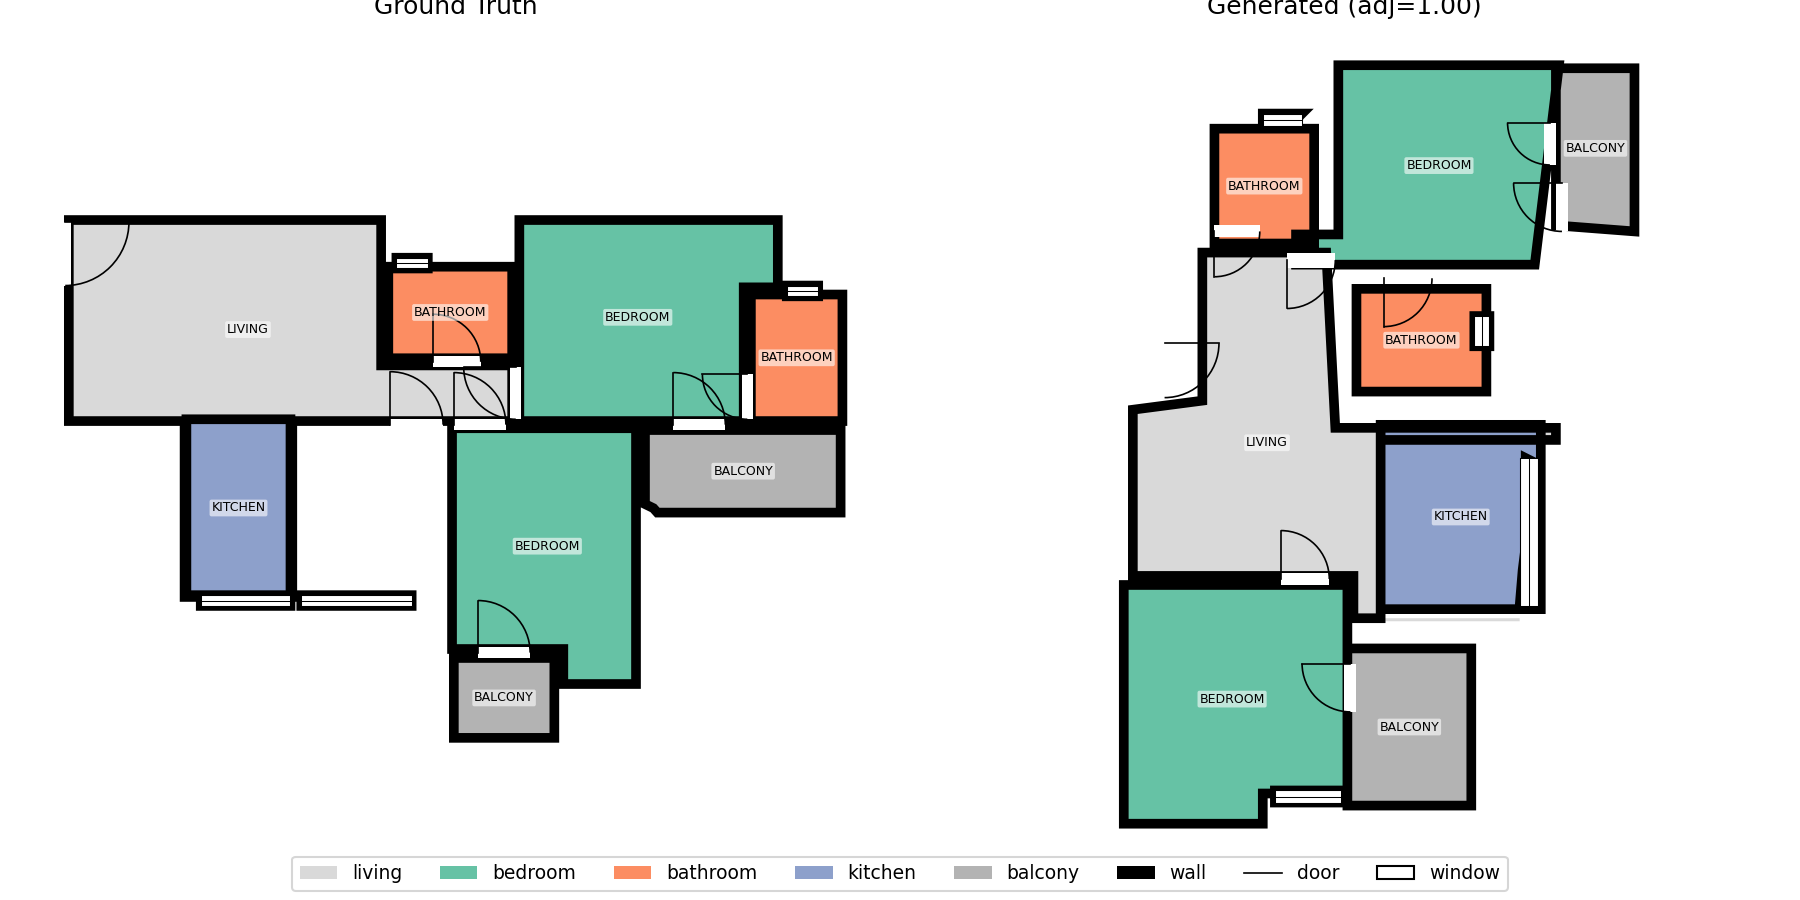
\includegraphics[width=\linewidth]{figures/qual_sample_a.png}\\[2pt]
  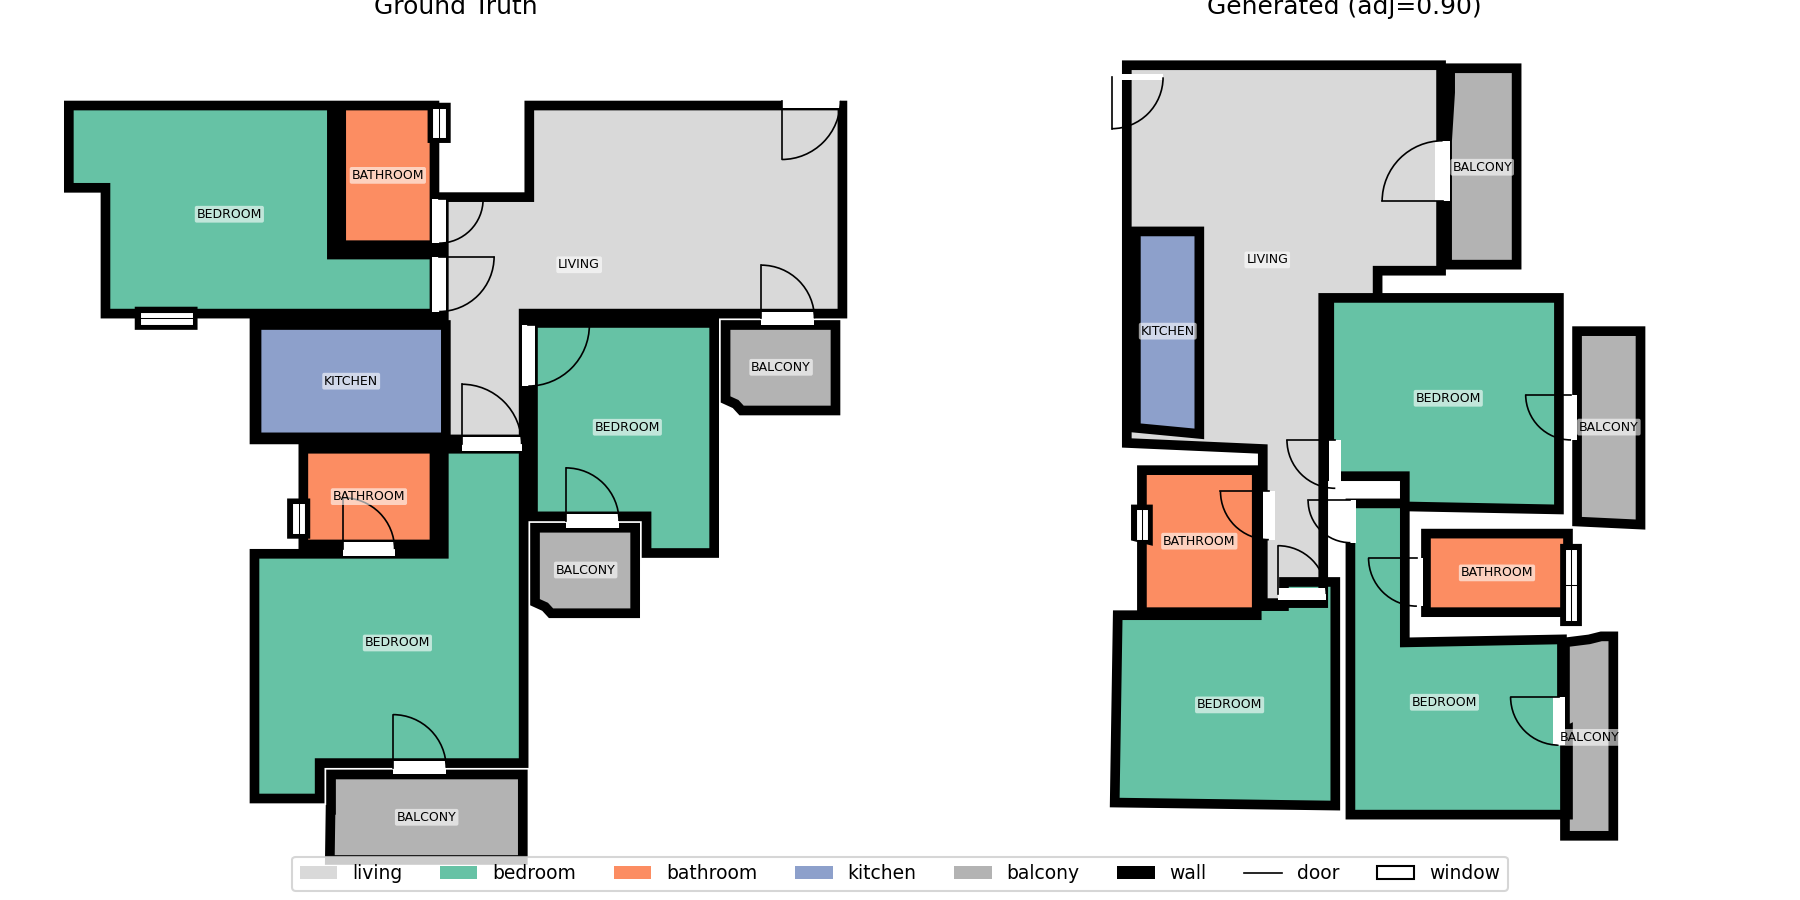
\includegraphics[width=\linewidth]{figures/qual_sample_b.png}
  \caption{Qualitative comparison on two held-out plans: ground truth (left) and a
  sample from the final model (right), drawn with the architectural renderer. The
  generated layouts match the conditioning rooms and adjacencies; geometry is the
  weaker point.}
  \label{fig:qualitative}
\end{figure}
